% Template for ICASSP-2016 paper; to be used with:
%          spconf.sty  - ICASSP/ICIP LaTeX style file, and
%          IEEEbib.bst - IEEE bibliography style file.
% --------------------------------------------------------------------------
\documentclass{article}
\setlength{\parindent}{0pt}
\usepackage{spconf,amsmath,graphicx}
\usepackage{tikz}
\usetikzlibrary{calc,chains,shapes,positioning}
\usepackage{phaistos}
\usepackage{pgfplots}
\usepackage{tabularx}
\usepackage{booktabs}
\usepackage{cite}
% \usetikzlibrary{external}
% \tikzexternalize
%\usepackage[subtle]{savetrees}
% Example definitions.
% --------------------
\def\x{{\mathbf x}}
\def\L{{\cal L}}
\def\ninept{\def\baselinestretch{.9}\let\normalsize\small\normalsize}
% Title.
% ------
\title{Robust Sparsity-promoting acoustic multi-channel equalization \\ for speech dereverberation}
%
% Single address.
% ---------------
% Single address.
% ---------------
\name{Ina Kodrasi, Ante Juki\'{c}, Simon Doclo
\thanks{
This work was supported by a Grant from the GIF, the German-Israeli Foundation for Scientific
Research and Development, the Cluster of Excellence 1077 ``Hearing4All'', funded by the German Research Foundation (DFG), and the Marie Curie Initial Training Network DREAMS (Grant no. 316969).
}}
\address{
University of Oldenburg, Department of Medical Physics and Acoustics, \\ and Cluster of Excellence Hearing4All, Oldenburg, Germany \\
{\tt ina.kodrasi@uni-oldenburg.de}\\
}

\begin{document}
\newlength\figureheight
\newlength\figurewidth
\setlength\figureheight{2cm}
\setlength\figurewidth{0.3\columnwidth}
\ninept
%
\maketitle
%
\begin{abstract}
This paper presents a novel signal-dependent method to increase the robustness of acoustic multi-channel equalization  techniques against room impulse response (RIR) estimation errors.
Aiming at obtaining an output signal which better resembles a clean speech signal, we propose to extend the acoustic multi-channel equalization cost function with a penalty function which promotes sparsity of the output signal in the short-time Fourier transform domain.
Two conventionally used sparsity-promoting penalty functions are investigated, i.e., the $l_0$-norm and the $l_1$-norm, and the sparsity-promoting filters are iteratively computed using the alternating direction method of multipliers.
Simulation results for several RIR estimation errors show that incorporating a sparsity-promoting penalty function significantly increases the robustness, with the $l_1$-norm penalty function outperforming the $l_0$-norm penalty function.

\end{abstract}
%
\begin{keywords}
speech dereverberation, sparsity, robustness, RIR estimation errors
\end{keywords}
%
\section{Introduction}
\label{sec: intro}
Acoustic multi-channel equalization techniques aim at speech dereverberation by reshaping the estimated room impulse responses (RIRs) between the speech source and the microphone array~\cite{Miyoshi_ITASS_1988,Kallinger_ICASSP_2006,Kodrasi_ITASLP_2013,Lim_ITASLP_2014}.
Although in theory perfect dereverberation can be achieved when multiple microphones are available~\cite{Miyoshi_ITASS_1988}, such an approach poses the practical challenge of achieving robustness against errors in the estimated RIRs~\cite{Hikichi_EURASIP_2007,Kodrasi_ITASLP_2013,Lim_ITASLP_2014}. 
Since the estimated RIRs typically differ from the true RIRs~\cite{Radlovic_ITSA_2000,Hasan_EUSIPCO_2006}, acoustic multi-channel equalization techniques may fail to achieve dereverberation and may cause distortions in the output signal~\cite{Radlovic_ITSA_2000,Kodrasi_ITASLP_2013}. 

Several methods have been proposed to increase the robustness of equalization techniques against RIR estimation errors, such as, e.g., relaxing the constraints on the filter design by using a weighted least-squares or an energy-based optimization criterion~\cite{Kallinger_ICASSP_2006,Lim_ITASLP_2014}, incorporating regularization to reduce the filter energy~\cite{Hikichi_EURASIP_2007,Kodrasi_ITASLP_2013}, or using a shorter filter length to improve the conditioning of the underlying optimization criteria~\cite{Kodrasi_EUSIPCO_2012}.
To the best of our knowledge, all proposed methods are {\textit{signal-independent}} methods, i.e., they rely only on the estimated RIRs for the filter design, without incorporating knowledge of the resulting output signal.

In this paper we propose a {\textit{signal-dependent}} method to increase the robustness of equalization techniques by incorporating the output signal in the filter design, with the aim of enforcing it to exhibit spectro-temporal characteristics of a clean speech signal.
Given the successful exploitation of the sparse nature of clean speech in several speech enhancement techniques~\cite{makino_2010,Kameoka_ICASSP_2009,vanwaterschoot13-122,Jukic_ITASLP_2015}, we propose to promote sparsity of the output signal in the short-time Fourier transform~(STFT) domain by extending the acoustic multi-channel equalization cost function with an $l_0$-norm or $l_1$-norm penalty function.
% Exploiting the sparse nature of clean speech signals has proven to be beneficial in many speech enhancement techniques, such as in underdetermined blind source separation~\cite{}, adaptive beamforming~\cite{}, and blind single- or multi-channel dereverberation techniques~\cite{}.
The sparsity-promoting filters are iteratively computed using the alternating direction method of multipliers~(ADMM), since it is a well-suited algorithm for solving large scale problems with sparsity-promoting penalty functions~\cite{Boyd_admm_2011}.
Simulation results show that promoting sparsity of the output signal significantly increases the robustness of equalization techniques against RIR estimation errors, with the $l_1$-norm penalty function outperforming the $l_0$-norm penalty function.

\section{Configuration and Notation}
\label{sec: configuration}
Consider the acoustic system depicted in Fig.~\ref{fig: conf}, consisting of a single speech source and $M$ microphones. 
\begin{figure}[b!]
  \centering
  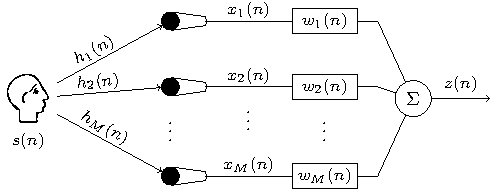
\includegraphics[scale=0.7]{config}
  \caption{Acoustic system configuration.}
  \label{fig: conf}
\end{figure}
The $m$-th microphone signal $x_m(n)$ at time index $n$ is given by
\begin{equation}
x_m(n) = s(n) \ast h_m(n), \; \; \; \; \; \; \; \; m = 1, \; \; \ldots, \; \; M,
\vspace{-0.15cm}
\end{equation}
with $s(n)$ the clean speech signal, $h_m(n)$ the RIR between the speech source and the $m$-th microphone, and $\ast$ denoting convolution.
Using the filter-and-sum structure in Fig.~\ref{fig: conf}, the output signal $z(n)$ is equal to the sum of the filtered microphone signals, i.e.,
\begin{equation}
\label{eq: out_sig}
z(n) = \sum_{m=1}^M x_m(n) \ast w_m(n) = s(n) \ast \underbrace{\sum_{m=1}^M h_m(n) \ast w_m(n)}_{c(n)},
\vspace{-0.15cm}
\end{equation}
with $w_m(n)$ the filter applied to the $m$-th microphone signal and $c(n)$ the equalized impulse response~(EIR) between the speech source and the output of the system.
In vector notation, the RIR $\mathbf{h}_m$ and the filter $\mathbf{w}_m$ are given by
\begin{align}
\!\!\!\!\mathbf{h}_m & \!=\! [h_m(0)  \ldots  h_m(L_h\!\!-\!\!1)]^T\!\!\!, \;\mathbf{w}_m \!=\! [w_m(0) \ldots w_m(L_w\!\!-\!\!1)]^T\!\!, \!\!\!\!
\end{align}
where $L_h$ and $L_w$ denote the RIR length and the filter length, respectively.
Furthermore, the $L_c$-dimensional EIR vector $\mathbf{c}$, with $L_c = L_h+L_w-1$, is given by $\mathbf{c} = [c(0) \ldots c(L_c-1)]^T$.
Using the $ML_w$-dimensional stacked filter vector $\mathbf{w} = [\mathbf{w}^T_1 \ldots  \mathbf{w}^T_M]^T$ and the $L_c \times ML_w$-dimensional multi-channel convolution matrix of the RIRs $\mathbf{H} = [\mathbf{H}_1 \ldots \mathbf{H}_M]$, with $\mathbf{H}_m$ the $L_c \times L_w$-dimensional convolution matrix of $\mathbf{h}_m$, the output signal in~(\ref{eq: out_sig}) can be expressed as
\begin{equation}
\label{eq: outsig_vec}
z(n) = \sum_{m=1}^M \mathbf{w}_m^T\underbrace{\mathbf{H}^T_m\mathbf{s}(n)}_{\mathbf{x}_m(n)} = \underbrace{\mathbf{w}^T\mathbf{H}^T}_{\mathbf{c}^T}\mathbf{s}(n),
\end{equation}
with $\mathbf{s}(n) = [s(n) \ldots s(n-L_c+1)]^T$ the $L_c$-dimensional clean speech vector, $\mathbf{x}_m(n) = [x_m(n) \ldots x_m(n-L_w+1)]^T$ the $L_w$-dimensional signal vector at the $m$-th microphone, and
\begin{equation}
\label{eq: eir_vec}
\mathbf{c} = \mathbf{H}\mathbf{w}.
\end{equation}
Alternatively, the output signal in~(\ref{eq: outsig_vec}) can also be expressed as
\begin{equation}
\label{eq: outsig_vecalter}
z(n) = \sum_{m=1}^M \mathbf{x}_m^T(n)\mathbf{w}_m = \mathbf{x}^T(n)\mathbf{w},
\end{equation}
with $\mathbf{x}(n) = [\mathbf{x}^T_1(n) \ldots \mathbf{x}^T_M(n)]^T$ the $ML_w$-dimensional stacked signal vector.
Based on~(\ref{eq: outsig_vecalter}), the $L_z$-dimensional output signal vector $\mathbf{z}(n) = [z(n) \ldots z(n-L_z+1)]^T$ can be written as
\begin{equation}
\mathbf{z}(n) = \mathbf{X}(n)\mathbf{w},
\end{equation}
with $\mathbf{X}(n)$ the $L_z \times ML_w$-dimensional multi-channel convolution matrix of the microphone signals, i.e.,  $ \mathbf{X}(n) = [\mathbf{X}_1(n) \ldots \mathbf{X}_M(n)]$, where $\mathbf{X}_m(n)$ denotes the $L_z\times L_w$-dimensional convolution matrix of $\mathbf{x}_m(n)$.
For conciseness, the time index $n$ will be omitted when possible in the remainder of this paper.

\section{Acoustic Multi-Channel Equalization}

\label{sec: equalization}
Acoustic multi-channel equalization techniques aim at speech dereverberation by designing the filter $\mathbf{w}$ such that the resulting EIR $\mathbf{c}$ in~(\ref{eq: eir_vec}) resembles a dereverberated target EIR $\mathbf{c}_t$.
Since the true RIRs are generally not available in practice~\cite{Radlovic_ITSA_2000,Hasan_EUSIPCO_2006}, such techniques design $\mathbf{w}$ using the estimated multi-channel convolution matrix $\hat{\mathbf{H}}$~(constructed from the estimated RIRs $\hat{\mathbf{h}}_m$) instead of the true multi-channel convolution matrix $\mathbf{H}$.

In this paper we will focus on the partial multi-channel equalization technique based on the multiple-input/output inverse theorem~(PMINT) proposed in~\cite{Kodrasi_ITASLP_2013}, which has been shown to be a perceptually advantageous technique.
%\footnote{Note that the method proposed in this paper can also be applied to increase the robustness of other acoustic multi-channel equalization techniques.}.
The PMINT technique aims at simultaneously suppressing late reverberation and preserving perceptual speech quality by using a target EIR $\mathbf{c}_t$ whose late reflection taps are equal to $\mathbf{0}$, while the remaining taps are equal to the direct path and early reflections of one of the estimated RIRs, i.e.,
\begin{equation}
\label{eq: eir_tar}
\mathbf{c}_t = [\hat{h}_q(0) \ldots \hat{h}_q(L_d-1) \; 0 \ldots 0]^T,
\end{equation}
with $L_d$ the length of the direct path and early reflections and $q \in \{1, \; \ldots, \; M \}$.
The PMINT filter is computed by minimizing the least-squares cost function
\begin{equation}
\label{eq: cost_p}
J_{_{\text{P}}}(\mathbf{w}) = \|\hat{\mathbf{H}}\mathbf{w} - \mathbf{c}_t \|_2^2.
\end{equation}
As shown in~\cite{Miyoshi_ITASS_1988,Kodrasi_ITASLP_2013}, assuming that the RIRs do not share any common zeros and using $L_w \geq \left\lceil{\frac{L_h-1}{M-1}}\right\rceil$, with $\left\lceil{\cdot}\right\rceil$ the ceiling operator, the PMINT filter minimizing the cost function in~(\ref{eq: cost_p}) is equal to
\begin{equation}
\label{eq: w_pmint}
\mathbf{w}_{_{\text{P}}} = \hat{\mathbf{H}}^+\mathbf{c}_t,
\end{equation}
where $\{ \cdot \}^+$ denotes the matrix pseudo-inverse. 
When the true RIRs are available, i.e., $\hat{\mathbf{H}} = \mathbf{H}$, the PMINT filter yields perfect dereverberation performance, i.e., $\mathbf{H}\mathbf{w}_{_{\text{P}}} = \mathbf{c}_t$~\cite{Kodrasi_ITASLP_2013}.
However, in the presence of RIR estimation errors, i.e., $\hat{\mathbf{H}} \neq \mathbf{H}$, the PMINT filter fails to achieve dereverberation, i.e., $\mathbf{H}\mathbf{w}_{_{\text{P}}} \neq \mathbf{c}_t$, causing distortions in the output signal~\cite{Kodrasi_ITASLP_2013}.

Several methods have been proposed to increase the robustness of equalization techniques against RIR estimation errors, e.g., relaxing the constraints on the filter design using a weighted least-squares or an energy-based optimization criterion~\cite{Kallinger_ICASSP_2006,Lim_ITASLP_2014}, incorporating regularization~\cite{Hikichi_EURASIP_2007,Kodrasi_ITASLP_2013}, or decreasing the filter length $L_w$~\cite{Kodrasi_EUSIPCO_2012}.
To the best of our knowledge, all proposed methods are {\textit{signal-independent}} methods, i.e., they only use the estimated convolution matrix $\hat{\mathbf{H}}$ for the filter design without incorporating knowledge of the resulting output signal $\mathbf{z}$.
The objective of this paper is to explore the potential of increasing the robustness of acoustic multi-channel equalization techniques by incorporating a {\textit{signal-dependent}} penalty function, which enforces the output signal $\mathbf{z}$ to exhibit spectro-temporal characteristics of a clean speech signal. Although the proposed method is discussed as an extension of the PMINT technique, it can also be applied to increase the robustness of other (more robust and signal-independent) acoustic multi-channel equalization techniques.

\section{Sparsity-Promoting \\ Acoustic Multi-Channel Equalization}
\label{sec: sparsity}

While in principle any well-defined characteristic of clean speech could be exploited, we propose to use a penalty function which promotes sparsity of the output signal in the STFT domain.
The advantage of promoting sparsity of the output signal is expected to be twofold.
First, it is widely accepted that clean speech is sparse in the STFT domain~\cite{makino_2010,Tashev_IWAENC_2010,Gerkmann_IWAENC_2010}. 
Empirical observations, e.g., in~\cite{makino_2010}, have shown that when clean speech is corrupted by reverberation (and noise), the STFT coefficients are less sparse than the STFT coefficients of clean speech.
Hence, promoting sparsity of the output signal yields a signal which better resembles a clean speech signal.
% In the presence of reverberation, the pauses between phonemes and the formant transitions in voiced sounds, i.e., the (nearly) zero energy STFT coefficients of the clean speech signal, are filled with reverberant energy, making the reverberant STFT coefficients less sparse than the clean speech STFT coefficients.
Second, in the presence of RIR estimation errors, non-robust equalization techniques introduce distortions (i.e., non-zero STFT coefficients) in the output signal~\cite{Kodrasi_ITASLP_2013}.
By sparsifying the STFT representation of the output signal it is expected that these distortions are reduced.
% Exploiting the sparse nature of clean speech signals has proven to be beneficial in many speech enhancement techniques, such as in under-determined blind source separation~\cite{}, adaptive beamforming~\cite{}, and single- or multi-channel dereverberation~\cite{}. 
% In the context of dereverberation, in~\cite{} a probabilistic modeling-based single-channel technique has been proposed, where dereverberation is achieved using an iterative algorithm to compute a filter that yields a sparse output speech signal in the STFT domain. 
% In~\cite{} a blind multi-channel speech dereverberation technique has been investigated, which jointly estimates the clean speech signal and the RIRs, exploiting the sparse nature of the clean speech STFT coefficients and a statistical reverberation model
% for the RIRs. 
% Furthermore, in~\cite{} it has been shown that the dereverberation performance of the conventional probabilistic modeling-based multi-channel linear prediction technique~\cite{} can be improved by modeling the dereverberated speech signal using a sparse prior.
% Motivated by the successful exploitation of the sparse nature of clean speech in several speech enhancement techniques, we propose to increase the robustness of acoustic multi-channel equalization techniques by taking into account the sparsity of the output speech signal STFT coefficients in the filter design.
\subsection{Cost function formulation}
The STFT coefficients of the output signal are computed as
\begin{equation}
Z(k,l) = \sum_{n=0}^{K-1}w_{_{\text{STFT}}}(n)z(lR+n)e^{-\frac{j 2 \pi k n}{K}},
\end{equation}
where $k = 0, \; \ldots, \; K\!-\!1$, denotes the frequency bin index with $K$ the frame size, $l = 0, \; \ldots, \; L-1$, denotes the frame index with $L$ the total number of frames, $w_{_{\text{STFT}}}(n)$ denotes the STFT analysis window, and $R$ denotes the frame shift. 
Similarly as in~\cite{Kowalski_ITASLP_2010}, we define the STFT operator $\boldsymbol{\Psi} \in {\cal{C}}^{L_{\tilde{z}}\times L_z}$ which transforms the $L_z$-dimensional time-domain vector $\mathbf{z}$ into the $L_{\tilde{z}}$-dimensional frequency-domain vector $\tilde{\mathbf{z}}$, i.e., $ \tilde{\mathbf{z}}= \boldsymbol{\Psi}\mathbf{z}$, consisting of all STFT coefficients $Z(k,l)$, with $L_{\tilde{z}} = K \times L$ (i.e., $\tilde{\mathbf{z}}$ denotes the stacked vector of the columns of the spectrogram of $\mathbf{z}$).
When using a tight STFT analysis window, the inverse STFT operator $\boldsymbol{\Psi}^H \in {\cal{C}}^{L_z \times L_{\tilde{z}}}$ is such that $\boldsymbol{\Psi}^H\boldsymbol{\Psi} = \mathbf{I}$, with $\mathbf{I}$ the $L_z \times L_z$-dimensional identity matrix.

The proposed sparsity-promoting PMINT cost function is then defined by adding a penalty function to~(\ref{eq: cost_p}), i.e.,
\begin{equation}
\label{eq: cost_sp}
J_{_{\text{S-P}}}(\mathbf{w}) = J_{_{\text{P}}}(\mathbf{w}) + \eta f_{_{\text{S}}}(\tilde{\mathbf{z}}) = \|\hat{\mathbf{H}}\mathbf{w}-\mathbf{c}_t \|_2^2 + \eta f_{_{\text{S}}}(\boldsymbol{\Psi}\mathbf{X}\mathbf{w}),
\end{equation}
with $f_{_{\text{S}}}(\tilde{\mathbf{z}})$ a sparsity-promoting penalty function and $\eta$ a weighting parameter providing a trade-off between the minimization of the least-squares error and the sparsity of the STFT coefficients of the output signal.
For the penalty function $f_{_{\text{S}}}(\tilde{\mathbf{z}})$, we propose two commonly used sparsity-promoting norms, i.e., the $l_0$-norm\footnote{Note that the $l_0$-norm is not a norm in the strict mathematical sense, since it does not satisfy all properties of a norm.} $f_{_{\text{S}}}^0(\tilde{\mathbf{z}})$ and the $l_1$-norm $f_{_{\text{S}}}^1(\tilde{\mathbf{z}})$, defined as
\begin{equation}
\label{eq: l0_norm}
f_{_{\text{S}}}^0(\tilde{\mathbf{z}}) = |i: \tilde{z}(i) \neq 0 |,  \; \; \;  \; \; \; f_{_{\text{S}}}^1(\tilde{\mathbf{z}}) = \sum_{i=0}^{L_{\tilde{z}}-1}|\tilde{z}(i)|,
\end{equation}
with the $l_1$-norm differing from the $l_0$-norm by penalizing the large coefficients of $\tilde{\mathbf{z}}$ more than the small coefficients. 
It should be noted that the $l_0$-norm is non-convex and it is well known that optimization problems with non-convex penalty functions are typically hard (if not impossible) to solve exactly, particularly for large scale problems~\cite{Natarajan_SIAM_1995}. 
The $l_1$-norm on the other hand can be viewed as a convex relaxation of the $l_0$-norm, and efficient methods have been proposed to solve optimization problems with $l_1$-norm penalty functions~\cite{Boyd_book,Chartrand_ICASSP_2014}. 
% Furthermore, it has been shown that under certain conditions, replacing the $l_0$-norm by the $l_1$-norm provides the solution to the original $l_0$-norm optimization problem~\cite{}. 
% In practice however, the $l_1$-norm relaxation is very often used when these conditions are not satisfied, typically resulting in a solution which does not optimize the original $l_0$-norm optimization problem, but nevertheless provides smaller $l_0$-norm values.
\subsection{Cost function optimization based on the alternating direction method of multipliers~(ADMM)}
Since no closed-form expression is available for the filter minimizing the cost function in~(\ref{eq: cost_sp}), iterative optimization algorithms are required.
%As a result, there has been much research in the development of efficient iterative optimization algorithms for solving convex as well as non-convex optimization problems. 
We have chosen to use the ADMM algorithm, since it is a well-suited algorithm for solving large scale optimization problems of the form in~(\ref{eq: cost_sp})~\cite{Boyd_admm_2011}.
Within the ADMM framework, the minimization of the sparsity-promoting cost function in~(\ref{eq: cost_sp}) is reformulated as
\begin{equation}
\label{eq: cost_reform}
\min_{\mathbf{w}} \left[ \|\hat{\mathbf{H}}\mathbf{w}-\mathbf{c}_t \|_2^2 + \eta f_{_{\text{S}}}(\tilde{\mathbf{a}}) \right] \; \; {\text{subject to}} \; \; \boldsymbol{\Psi}\mathbf{X}\mathbf{w} = \tilde{\mathbf{a}},
\end{equation}
introducing the auxiliary variable $\tilde{\mathbf{a}}$ such that the optimization problem in~(\ref{eq: cost_sp}) can be split into simpler sub-problems.
The augmented Lagrangian of~(\ref{eq: cost_reform}) is equal to
\begin{equation}
\label{eq: lag}
{\cal{L}} = \|\hat{\mathbf{H}}\mathbf{w}-\mathbf{c}_t \|_2^2 + \eta f_{_{\text{S}}}(\tilde{\mathbf{a}}) + \frac{\rho}{2} \|\boldsymbol{\Psi}\mathbf{X}\mathbf{w} +\boldsymbol{\lambda} - \tilde{\mathbf{a}}\|_2^2,
\end{equation}
with $\boldsymbol{\lambda}$ the $L_{\tilde{z}}$-dimensional dual variable and $\rho>0$ the penalty parameter.
The ADMM algorithm minimizes~(\ref{eq: lag}) alternately with respect to the variables $\mathbf{w}$ and $\tilde{\mathbf{a}}$, followed by a dual ascent over the variable $\boldsymbol{\lambda}$.
The ADMM update rules are given by:
{\small{\begin{align}
\label{eq: upw}
\!\!\mathbf{w}^{(i+1)} & \!=\! \underset{\mathbf{w}}{\arg\min} \left[\|\hat{\mathbf{H}}\mathbf{w} \!-\! \mathbf{c}_t\|_2^2  \!+\! \frac{\rho}{2} \|\mathbf{\Psi}\mathbf{X}\mathbf{w} \!+\! \boldsymbol{\lambda}^{(i)} \!-\! \tilde{\mathbf{a}}^{(i)} \|_2^2 \right]\!\!, \!\!\! \\
\label{eq: upz}
\!\!\tilde{\mathbf{a}}^{(i+1)} & \!=\! \underset{\tilde{\mathbf{a}}}{\arg\min} \left[ \eta f_{\text{S}}(\tilde{\mathbf{a}}) \!+\! \frac{\rho}{2} \|\mathbf{\Psi}\mathbf{X}\mathbf{w}^{(i+1)} \!+\! \boldsymbol{\lambda}^{(i)} \!-\! \tilde{\mathbf{a}} \|_2^2 \right]\!\!, \\
\label{eq: up_lambda_sls}
\boldsymbol{\lambda}^{(i+1)} & \!=\! \boldsymbol{\lambda}^{(i)} \!+\! \mathbf{\Psi}\mathbf{X}\mathbf{w}^{(i+1)} \!-\! \tilde{\mathbf{a}}^{(i+1)},
\end{align}}}%
where $\{\cdot\}^{(i)}$ denotes the variable in the $i$-th iteration.
The original minimization problem in~(\ref{eq: cost_sp}) is hence decomposed into simpler sub-problems, which are solved in an alternating fashion using the update rules in~(\ref{eq: upw}),~(\ref{eq: upz}), and~(\ref{eq: up_lambda_sls}) until a convergence criterion is satisfied or a maximum number of iterations is exceeded~(cf. Section~\ref{sec: acsys}).
In the following, the update rules for the filter and the auxiliary variable in~(\ref{eq: upw}) and~(\ref{eq: upz}) are presented.

{\textit{1) Filter update rule:}} \enspace Minimizing~(\ref{eq: upw}) yields
{\small{\begin{equation}
\label{eq: w_admm_sls}
\!\mathbf{w}^{(i+1)} \!\!=\!\! (\underbrace{2 \hat{\mathbf{H}}^T\hat{\mathbf{H}} \!+\! \rho \mathbf{X}^T \mathbf{X}}_{\mathbf{C}})^{-1} [\underbrace{2 \hat{\mathbf{H}}^T \!\!\mathbf{c}_t}_{\mathbf{b}^{}_1} + \rho \underbrace{\mathbf{X}^T \mathbf{\Psi}^H \!(\tilde{\mathbf{a}}^{(i)} \!\!-\!\! \boldsymbol{\lambda}^{(i)})}_{\mathbf{b}_2^{(i)}}],\!\!\!\!
\end{equation}}}%
where the variables $\mathbf{C}$, $\mathbf{b}_1$, and $\mathbf{b}_2$ are introduced to highlight that only the variable $\mathbf{b}_2$ is iteration-dependent, whereas the variables $\mathbf{C}$ and $\mathbf{b}_1$ can be pre-computed.
Although~(\ref{eq: w_admm_sls}) appears to require a matrix inversion in each iteration, the filter update can be efficiently computed by, e.g., storing the LU-factorization of $\mathbf{C}$ and using forward and backward substitution.

{\textit{2) Auxiliary variable update rule:}} \enspace The solution to~(\ref{eq: upz}) is the proximal mapping of the sparsity-promoting penalty function, which exists in closed-form for the $l_0$- and $l_1$-norm penalty functions~\cite{Chartrand_ICASSP_2014,parikh2014proximal}.
Defining the variable $\mathbf{b}^{(i)}= \mathbf{\Psi}\mathbf{X}\mathbf{w}^{(i+1)} + \boldsymbol{\lambda}^{(i)}$ to simplify the notation, the proximal mapping for the $l_0$-norm is the element-wise {\textit{hard thresholding}} map, i.e.,
    \begin{equation}
      \label{eq: aux_up_l0}
      \tilde{a}_j^{(i+1)} =  \left(|b_j^{(i)}| - \frac{\eta}{\rho} \right)_+ \frac{b_j^{(i)}}{|b_j^{(i)}| - \frac{\eta}{\rho}},
    \end{equation}
    with $\{ \cdot \}_j$ denoting the $j$-th element of a vector and $\left(T \right)_{+} = \max (T,0)$.
    The proximal mapping for the $l_1$-norm penalty function is the element-wise {\textit{soft thresholding}} map, i.e.,
    \begin{equation}
      \label{eq: aux_up_l1}
      \tilde{a}_j^{(i+1)} = \left( |b_j^{(i)}| - \frac{\eta}{\rho} \right)_+\frac{b_j^{(i)}}{|b_j^{(i)}|}.
    \end{equation}
In summary, using the filter update rule in~(\ref{eq: w_admm_sls}), the auxiliary variable update rule in~(\ref{eq: aux_up_l0}) or~(\ref{eq: aux_up_l1}), and the dual variable update rule in~(\ref{eq: up_lambda_sls}) until a termination criterion is satisfied, the sparsity-promoting PMINT filter can be computed.

\begin{figure*}[t!]
  \centering
  % This file was created by matlab2tikz v0.4.0.
% Copyright (c) 2008--2013, Nico Schlömer <nico.schloemer@gmail.com>
% All rights reserved.
% 
% The latest updates can be retrieved from
%   http://www.mathworks.com/matlabcentral/fileexchange/22022-matlab2tikz
% where you can also make suggestions and rate matlab2tikz.
% 
% 
% 
\begin{tikzpicture}[font=\small]

\begin{axis}[%
width=\figurewidth,
height=\figureheight,
axis on top,
scale only axis,
xmin=0,
xmax=3.12,
ymin=-7.8125,
xlabel style = {text width=1.55cm,align=center},
xlabel = {Time [s] \\ (a)},
xlabel style={yshift=0.8em},
ymax=4007.8125,
ylabel={Frequency [kHz]},
ylabel absolute, ylabel style={yshift=-2.0em},
ytick = {0,1000,2000,3000,4000},
yticklabels = {0,1,2,3,4},
colormap/jet,
%colorbar,
point meta min=-120,
point meta max=-40
]
\addplot graphics [xmin=0.016,xmax=3.12,ymin=-7.8125,ymax=4007.8125] {Plots/spec_sd-1.png};
\end{axis}
%\draw[opacity=0] (current bounding box.north west) rectangle
%([xshift=20pt] current bounding box.south east);
\end{tikzpicture}% % This file was created by matlab2tikz v0.4.0.
% Copyright (c) 2008--2013, Nico Schlömer <nico.schloemer@gmail.com>
% All rights reserved.
% 
% The latest updates can be retrieved from
%   http://www.mathworks.com/matlabcentral/fileexchange/22022-matlab2tikz
% where you can also make suggestions and rate matlab2tikz.
% 
% 
%
\begin{tikzpicture}[font=\small]

\begin{axis}[%
width=0.6\figurewidth,
height=1\figureheight,
axis on top,
scale only axis,
xmin=0,
xmax=3,
ymin=-7.8125,
xlabel style = {text width=1.55cm,align=center},
xlabel = {Time $t$ [s] \\ (b)},
xlabel style={yshift=0.5em},
ymax=4007.8125,
%ylabel={Frequency $f$ [kHz]},
%ylabel absolute, ylabel style={yshift=-2.0em},
%ytick = {0,1000,2000,3000,4000},
yticklabels = {},
colormap/jet,
%colorbar,
point meta min=-120,
point meta max=-40
]
\addplot graphics [xmin=0.016,xmax=3.056,ymin=-7.8125,ymax=4007.8125] {Plots/spec_rev-1.png};
\end{axis}
\end{tikzpicture}% % This file was created by matlab2tikz v0.4.0.
% Copyright (c) 2008--2013, Nico Schlömer <nico.schloemer@gmail.com>
% All rights reserved.
% 
% The latest updates can be retrieved from
%   http://www.mathworks.com/matlabcentral/fileexchange/22022-matlab2tikz
% where you can also make suggestions and rate matlab2tikz.
% 
% 
%
\begin{tikzpicture}[font=\small]

\begin{axis}[%
width=0.6\figurewidth,
height=1\figureheight,
axis on top,
scale only axis,
xmin=0,
xmax=3,
ymin=-7.8125,
xlabel style = {text width=1.55cm,align=center},
xlabel = {Time $t$ [s] \\ (c)},
xlabel style={yshift=0.5em},
ymax=4007.8125,
%ylabel={Frequency [kHz]},
%ylabel absolute, ylabel style={yshift=-2.0em},
ytick = {0,1000,2000,3000,4000},
yticklabels = {},
colormap/jet,
colorbar,
colorbar style={
font = \footnotesize,
at={(1.05,0)},anchor=south west},
%colorbar,
point meta min=-120,
point meta max=-40
]
\addplot graphics [xmin=0.016,xmax=3.056,ymin=-7.8125,ymax=4007.8125] {Plots/spec_pmint-1.png};
\end{axis}
\end{tikzpicture}% % This file was created by matlab2tikz v0.4.0.
% Copyright (c) 2008--2013, Nico Schlömer <nico.schloemer@gmail.com>
% All rights reserved.
% 
% The latest updates can be retrieved from
%   http://www.mathworks.com/matlabcentral/fileexchange/22022-matlab2tikz
% where you can also make suggestions and rate matlab2tikz.
% 
% 
% 
\begin{tikzpicture}[font = \small]

\begin{axis}[%
width=\figurewidth,
height=\figureheight,
axis on top,
scale only axis,
xmin=0,
xmax=3.12,
xlabel style = {text width=1.55cm,align=center},
xlabel = {Time [s] \\ (d)},
xlabel style={yshift=0.8em},
ytick = {0,1000,2000,3000,4000},
yticklabels = {0,1,2,3,4},
ymin=-7.8125,
ymax=4007.8125,
colormap/jet,
%colorbar,
point meta min=-120,
point meta max=-40
]
\addplot graphics [xmin=0.016,xmax=3.12,ymin=-7.8125,ymax=4007.8125] {Plots/spec_l0-1.png};
\end{axis}
\end{tikzpicture}% % This file was created by matlab2tikz v0.4.0.
% Copyright (c) 2008--2013, Nico Schlömer <nico.schloemer@gmail.com>
% All rights reserved.
% 
% The latest updates can be retrieved from
%   http://www.mathworks.com/matlabcentral/fileexchange/22022-matlab2tikz
% where you can also make suggestions and rate matlab2tikz.
% 
% 
% 
\begin{tikzpicture}[font = \small]

\begin{axis}[%
width=\figurewidth,
height=\figureheight,
axis on top,
scale only axis,
xmin=0,
xmax=3.12,
xlabel={Time [s]},
ymin=-7.8125,
ymax=4007.8125,
xlabel style = {text width=1.55cm,align=center},
xlabel = {Time [s] \\ (e)},
xlabel style={yshift=0.8em},
ytick = {0,1000,2000,3000,4000},
yticklabels = {0,1,2,3,4},
colormap/jet,
colorbar,
point meta min=-120,
point meta max=-40
]
\addplot graphics [xmin=0.016,xmax=3.12,ymin=-7.8125,ymax=4007.8125] {Plots/spec_l1-1.png};
\end{axis}
\end{tikzpicture}%
  \vspace{-0.7cm}
  \caption{Spectrogram of (a) reference signal $s_r(n)$, (b) input signal $x_1(n)$, and output signal $z(n)$ obtained using (c) PMINT, (d) $l_0$-PMINT, (e) $l_1$-PMINT (NPM $=-33$ dB).}
  \label{fig: spec}
\end{figure*}

\section{Simulations}
\label{sec: simulations}
In this section the dereverberation performance of the sparsity-promoting PMINT technique using the $l_0$- and $l_1$-norm penalty functions is compared to the PMINT technique for several RIR estimation errors.

\subsection{Algorithmic settings and performance measures}
\label{sec: acsys}
We consider an acoustic system with a single speech source and $M=4$ microphones in a room with reverberation time $T_{60} \approx 610$ ms~\cite{hadad_IWAENC_2014}. 
The source-microphone distance is $2$ m, the inter-microphone distance is $4$ cm, and the RIR length is $L_h = 4880$ at a sampling frequency of $8$ kHz.
To generate the microphone signals, $10$ sentences (approximately $17$ s long) from the HINT database~\cite{Nilsson_JASA_1994} have been convolved with the measured RIRs.

To simulate RIR estimation errors, the measured RIRs have been perturbed by adding scaled white noise as proposed in~\cite{Zhang_HINDAWI_2008}, such that a desired level of normalized projection misalignment~(NPM) between the true and the estimated RIRs is generated. 
The considered NPM values are ${\text{NPM}} \in \{-33~{\rm dB},  -27~{\rm dB}, -21~{\rm dB}, -15~{\rm dB}\}$. 

For all considered techniques the filter length is $L_w = 1600$ and the target response $\mathbf{c}_t$ is set to the direct path and early reflections of $\hat{\mathbf{h}}_1$, with the length of the direct path and early reflections corresponding to $10$ ms~(cf.~(\ref{eq: eir_tar})).
Furthermore, for the sparsity-promoting PMINT technique, the weighting and penalty parameters are empirically set to $\eta = 10^{-4}$ and $\rho = 10^{-1}$.

In order to reduce the computational complexity, the sparsity-promoting filters are computed using only the first $2$ sentences of the microphone signals (approximately $3$ s long). However, the complete output signal has been used for the evaluation. The STFT is computed using a $32$ ms Hamming window with $50$\% overlap between successive frames. The frame size is $K = 256$ and the total number of frames is $L = 208$.
For the ADMM algorithm, the variables $\mathbf{w}$, $\tilde{\mathbf{a}}$, and $\boldsymbol{\lambda}$ are initialized with $[1 \; 0 \ldots 0]^T$.
Furthermore, the termination criterion is set to either the number of iterations exceeding a maximum number of iterations or the relative change in the solution norm dropping below a tolerance, i.e.,
\begin{equation}
i + 1 > i_{\max} \; \; \; \; {\text{or}} \; \; \; \; \frac{\|\mathbf{w}^{(i+1)}-\mathbf{w}^{(i)}\|_2}{\|\mathbf{w}^{(i)}\|_2} < \epsilon,
\end{equation}
with $i_{\max} = 150$ and $\epsilon = 10^{-3}$.

The dereverberation performance is evaluated in terms of the reverberant energy suppression and the perceptual speech quality improvement.
The reverberant energy suppression is evaluated using the direct-to-reverberant-ratio improvement ($\Delta$DRR)~\cite{Naylor_Derev_book} between the resulting EIR $\mathbf{c}$ and the true RIR $\mathbf{h}_1$.
The improvement in perceptual speech quality is evaluated using the improvement in PESQ ($\Delta$PESQ)~\cite{PESQ} and in cepstral distance ($\Delta$CD)~\cite{Quackenbush_book} between the output signal $z(n)$ and the microphone signal $x_1(n)$. 
The reference signal $s_r(n)$ employed for PESQ and cepstral distance is the clean speech signal convolved with the direct path and early reflections of the true RIR $\mathbf{h}_1$.
It should be noted that an improvement in perceptual speech quality is indicated by a positive $\Delta$PESQ and a negative $\Delta$CD.

\subsection{Results}

Table~\ref{tbl: perf} presents the $\Delta$DRR, $\Delta$PESQ, and $\Delta$CD values obtained using the PMINT and the sparsity-promoting PMINT techniques with $l_0$-norm ($l_0$-PMINT) and $l_1$-norm ($l_1$-PMINT) penalty functions for several NPMs.
\begin{table}[t!]
\begin{center}
  \caption{Performance in terms of $\Delta$DRR, $\Delta$PESQ, and $\Delta$CD of the PMINT, $l_0$-PMINT, and $l_1$-PMINT techniques for several NPMs. The input DRR, PESQ, and CD are $-1.89$ dB, $2.15$, and $4.11$ dB.}
  \label{tbl: perf}
  \begin{tabularx}{\linewidth}{Xrrrr}
    \toprule
    NPM [dB] & $-33$ & $-27$ & $-21$ & $-15$ \\
    \midrule
    & \multicolumn{4}{c}{$\Delta$DRR [dB]} \\
    \midrule
    PMINT & $-18.47$ & $-18.16$ & $-17.43$ & $-15.41$ \\
    $l_0$-PMINT & $3.74$ & $2.76$ & $2.34$ & $0.22$ \\
    $l_1$-PMINT & ${\bf{8.15}}$ & $\bf{8.04}$ & $\bf{7.68}$ & $\bf{3.78}$ \\
    \midrule
    & \multicolumn{4}{c}{$\Delta$PESQ } \\
    \midrule
    PMINT & $-0.41$ & $-0.50$ & $-0.29$ & $-0.43$ \\
    $l_0$-PMINT & $0.07$ & $0.05$ & $-0.02$ & $-0.08$ \\
    $l_1$-PMINT & $\bf{0.36}$ & $\bf{0.42}$ & $\bf{0.32}$ & $\bf{0.03}$ \\
    \midrule
    & \multicolumn{4}{c}{$\Delta$CD [dB] } \\
    \midrule
    PMINT & $1.84$ & $1.96$ & $1.88$ & $1.90$ \\
    $l_0$-PMINT & $-0.68$ & $-0.29$ & $0.05$ & $0.39$ \\
    $l_1$-PMINT & $\bf{-0.90}$ & $\bf{-0.84}$ & $\bf{-0.50}$ & $\bf{0.14}$ \\
    \bottomrule
  \end{tabularx}
\end{center}
\vspace{-0.5cm}
\end{table}
It can be observed that, as expected, the PMINT technique fails to achieve dereverberation in the presence of RIR estimation errors and introduces distortions in the output signal, worsening the DRR, PESQ, and CD values.
Furthermore, it can be observed that incorporating the $l_0$-norm penalty function significantly improves the robustness of the PMINT technique, typically yielding  a slight improvement (for NPM $=-33$ dB and NPM $=-27$ dB) or a similar performance as the input signal (for NPM $=-21$ dB and NPM $=-15$ dB) in terms of all performance measures.
Finally, it can be observed that incorporating the $l_1$-norm penalty function yields the best performance in terms of the $\Delta$DRR, $\Delta$PESQ, and $\Delta$CD measures, outperforming the $l_0$-norm penalty function and resulting in a considerable improvement in comparison to the input signal.

To better illustrate the advantages of promoting sparsity of the output signal in the STFT domain, Fig.~\ref{fig: spec} presents the spectrograms of the reference signal $s_r(n)$, the microphone signal $x_1(n)$, and the output signal $z(n)$ obtained using the PMINT, $l_0$-PMINT, and $l_1$-PMINT techniques for an exemplary scenario of NPM $=-33$ dB.
Comparing Figs.~\ref{fig: spec}(a) and~\ref{fig: spec}(b), it can be observed that due to the spectro-temporal smearing effect of reverberation, the spectrogram of $x_1(n)$ is significantly less sparse than the spectrogram of $s_r(n)$.
Furthermore, Fig.~\ref{fig: spec}(c) shows that due to the distortions introduced in the output signal by the non-robust PMINT technique, the spectrogram of the output signal $z(n)$ obtained using PMINT is significantly less sparse than the spectrogram of $x_1(n)$.
On the contrary, Fig.~\ref{fig: spec}(d) shows that incorporating the $l_0$-norm penalty function sparsifies the spectrogram of the output signal, largely suppressing the distortions introduced by the PMINT technique as well as slightly suppressing the reverberant energy~(e.g., around $1$ kHz).
Finally, Fig.~\ref{fig: spec}(e) shows that incorporating the $l_1$-norm penalty function results in an even sparser spectrogram than the $l_0$-norm, significantly suppressing both the distortions introduced by the PMINT technique as well as the reverberant energy.

In summary, these simulation results confirm that incorporating a sparsity-promoting penalty function in equalization techniques yields a significant increase in robustness against RIR estimation errors. 
Incorporating such penalty functions in other (more robust signal-independent) equalization techniques as well as investigating other sparsity-promoting penalty functions, e.g., the weighted $l_1$-norm~\cite{Candes_FA_2008}, remain topics for future investigation.

\section{Conclusion}
In this paper we have presented a novel signal-dependent method to increase the robustness of acoustic equalization techniques against RIR estimation errors.
We have proposed to incorporate an $l_0$- and $l_1$-norm penalty function, aiming at promoting sparsity in the output signal and reducing distortions generated by non-robust equalization techniques.
The sparsity-promoting filters have been iteratively computed using the alternating direction method of multipliers.
Simulation results for several RIR estimation errors have validated the effectiveness of incorporating sparsity-promoting penalty functions to increase the robustness of equalization techniques, with the $l_1$-norm penalty function outperforming the $l_0$-norm penalty function.

% \section{REFERENCES}
% \label{sec:refs}

% References should be produced using the bibtex program from suitable
% BiBTeX files (here: strings, refs, manuals). The IEEEbib.bst bibliography
% style file from IEEE produces unsorted bibliography list.
% -------------------------------------------------------------------------
\bibliographystyle{IEEEbib}
\bibliography{strings,refs}

\end{document}
